\subsection{Skeletal Model}\label{subsec:2a}
The planar model representing the athletes body is torque actuated at five inelastic joints: ankle, knee, hips spine and shoulders.
Its Biorbd \cite{michaudBiorbd2021} representation has a floating base positioned at the feet \ref{fig:Model_Avatar} and is symmetric in the frontal plane, i.e. arm and leg segments represent both sides of the body.
Inertial parameters of the bodies were estimated from 95 anthropometric measurements of one subject (female, 21~years old, 65~kg, 158~cm) in line with Yeadon's anthropometric model~\cite{yeadon1990simulation}.
Joint torques were bounded to surfaces fitted on experimental maximal voluntary contractions acquired on one subject (male, ~years old, ~kg, ~cm)  as in [Allen2009 and Jackson2010].
\comEC{Comet est-ce que j'amène que la force de l'avatart c'est celles d'un homme plus grand/gros ?? Article Benjamin...}
\comEC{mention du pied actuator étrange ?}

\comEC{Fig model}
% \begin{figure}[h!]
% \centering
% \includegraphics[width=0.5\linewidth]{figures/Model_Final_2.png}
% \caption{Avatar model definition with 6 degrees-of-freedom: translations of the root ($q_{1-2}$), rotations of the root ($q_{3}$), knee flexion ($q_{4}$), hips flexion ($q_{5}$) and shoulder flexion ($q_{6}$)}
% \label{fig:Model_Avatar}
% \end{figure}


\subsection{Trampoline Model}\label{subsec:2b}
The model of the trampoline is composed of 15 mass-points and 38 ideal springs with constant characteristics in line with \cite{jacques2008determining} \ref{fig:Model_Toile}.
The outside extremity of contour springs are fixed to the trampoline frame.


\comEC{Fig model}
% \begin{figure}[h!]
% \centering
% \includegraphics[width=0.5\linewidth]{figures/Model_Final_2.png}
% \caption{Trampoline model with 15 point of mass $m_{1-15}$ and 38 springs of stiffness constant $k_{1-38}$.}
% \label{fig:Model_Toile}
% \end{figure}


\subsection{Determination of the trampoline force}\label{subsec:2c}

The force generated by the trampoline is accelerating at the same time the trampoline suspension system and the avatar.
Therefore the force acting on the avatar $F$ is proportional to the mass ratio of the avatar $m_{avatar}$ and the combined system $m_{trampoline} + m_{avatar}$.
It could be calculated with the following equation:
\[
F = \sum_{j=1}^{nb_{mass}=15} ( \sum_{h=1}^{nb_{adj}=4} k_h {(\ell_h - {\ell}^{relaxed}_h)} - m_j \mvec{g}p_{j_z}) ~ \frac{m_{avatar}}{m_{trampoline} + m_{avatar} }  \label{eq:Force_trampo}
\]

\noindent where ${k_h}$ the stiffness coefficient of the $h^{th}$ spring on the $j^{th}$ mass, $\ell_h$ the dimension of the $h^{th}$ spring on the $j^{th}$ mass, ${\ell}^{relaxed}_h$ the relaxed position of the $h^{th}$ spring on the $j^{th}$ mass, $m_j$ the mass of the $j^{th}$ mass-point,  $\mvec{g}$ the gravity vector and $p_{j_z}$ the z component of the $j^{th}$ mass-point position.
The constants in this equation are presented in Fig.~\ref{fig:Model_Toile}.
It also depends on variables which are the positions of the mass-points $\underline{\mvec{p}}$.
The deformation of the trampoline model was determined by static optimization.
The objective was to minimize the energy of the system (Eq. ~\ref{eq:min_energy}).
The position of the center point was imposed as a constraint to the optimization problem (Eq.~\ref{eq:const_pos_center}).
The problem was formulated as follow:  

\begin{subequations}
\begin{align}
 \underset{\substack{\underline{\mvec{p}}}}{\min} \hspace{2em} & \sum_{i=1}^{nb_{spring}=38} \dfrac{1}{2} k_i {(\ell_i - {\ell}^{relaxed}_i)}^{2} - \sum_{j=1}^{nb_{mass}=15} m_j g p_{j_z} \label{eq:min_energy} \\ 
   \st  \hspace{2em}  & p_{8} = p_{center} \label{eq:const_pos_center}
\end{align}
\end{subequations}

\noindent where $p_{center}$ is the defined position of the center mass-point.
The force computed in this section is composed of vertical and horizontal components, it is applied at the rear foot of the avatar.

% \subsection{Models interaction}\label{subsec:2d}
% The force generated by the trampoline calculated in Sec.~\ref{subsec:2c} is accelerating at the same time the trampoline suspension system and the avatar.
% Therefore the force acting on the avatar $F_{contact}$ is proportional to the mass ratio of the avatar $m_{avatar}$ and the combined system $m_{trampoline} + m_{avatar}$.
% \[
% F_{contact} = F  \frac{m_{avatar}}{m_{trampoline} + m_{avatar} }\label{eq:Force_contact}
% \]
% This force, composed of vertical and horizontal components is applied at the rear foot of the avatar.


\subsection{Formulation of the optimal control problem}\label{subsec:2e}
To address the different types of propulsion athletes can use in the case of non-twisting somersault, 4 types of optimal control problem (OCP) were formulated: forward somersaults from plain jump (F), backward somersaults from plain jump (B), forward somersaults from backward somersault (FB), backward somersaults from forward somersault (BF).
For each type of OCP, the number of somersaults ranged from 1 to 4, giving rise to the notation $F_2B_3$ for a movement composed of 2 forward somersaults in the preparation jump and 3 backward somersaults in the main jump.
The OCP were composed of 5 phases: bed depression of contact phase \#1, bed recoil of contact phase \#1, preparation jump, bed depression of contact phase \#2, bed recoil of contact phase \#2 and main somersaulting jump as presented in Fig.~\ref{fig:Model_phases}.
The main objective was to maximize the height reached by the CoM ($h_{CoM}$) during the flight phase of the two jumps (first term in Eq.~\ref{eq:ocp}).
The second ans third terms of Eq.~\ref{eq:ocp} were used to make sure the proper movement is executed.
The two last terms of Eq.~\ref{eq:ocp} are for control regularisation.
The objective was of the following form:

\[
 %\mathcal{J} = \alpha~(h_{CoM} \big\rvert_{t = t_3} + h_{CoM} \big\rvert_{t = t_6}) + \beta~(h_{bed} \big\rvert_{t = t_1} + h_{bed} \big\rvert_{t = t_4}) + \gamma~(\phi \big\rvert_{t = t_3} + % \phi \big\rvert_{t = t_6}) + \beta~\sum_{i=1}^{nb_{\tau}}  \int_0^T \tau_{i}^2 dt + \gamma~\sum_{i=1}^{nb_{\tau}}  \int_0^T \dot{\tau_{i}}^2 dt
\mathcal{J} = \alpha_1~(h_{CoM} \big\rvert_{t = t_3 \cup t_6}) + \alpha_2~(h_{bed} \big\rvert_{t = t_1 \cup t_4}) + \alpha_3~((\phi - \phi^*) \big\rvert_{t = t_3 \cup t_6}) + \alpha_4~\sum_{i=1}^{nb_{\tau}} \int_0^T \tau_{i}^2 dt + \alpha_5~\sum_{i=1}^{nb_{\tau}}  \int_0^T \dot{\tau_{i}}^2 dt \label{eq:ocp}
\]

\noindent where $\alpha_\cdot$ are the weighting coefficients listed in Table~\ref{Tab:weighting}, $h_{bed}$ is the bed depression, $\phi$ is the somersault rotation and $\phi^*$ is the targeted somersault rotation, T is the duration of the whole movement, $t_{\cdot}$ are the end time of the phases and $\tau_i$ is the torque actuation of the $i^{th}$ DoF.
\comEC{C'est wak d'écrire torque derivative comme ca :/}


Constraints were also added to make sure the task is executed in realistic conditions: 
\begin{itemize}
\item During the contact phases, the feet are attached to the center of the trampoline ($\tau_{1-2} = F(\underline{q})$).
\item Contact phases start and end when the feet pass ground level ($q_1 = 0$)
\item The range of motion, the velocity and the torques actuation of the joints are bounded to physiological values
\item ...
\end{itemize}
\comEC{C'est tu pertinent de laisser le bulletpoint avec réf à figure + mettre la forme éq dans la figure ? (pas trop le gout de faire une équation monstre)}


\begin{center}
\captionof{table}{Weighting coefficients of the OCP objective.}
\begin{tabular}{ c c }
 $\alpha_1$ & ... \\ 
 $\alpha_2$ & ... \\ 
 $\alpha_3$ & ... \\ 
 $\alpha_4$ & ... \\ 
 $\alpha_5$ & ... \\ 
 $\alpha_6$ & ...
\end{tabular}
\label{Tab:weighting}
\end{center}

\comEC{Figure pour illustrer les phases + objectifs associés + contraintes + phase transition ($T = t_1 + t_2 + t_3 + t_4 + t_5$)}
% \begin{figure}[h!]
% \centering
% 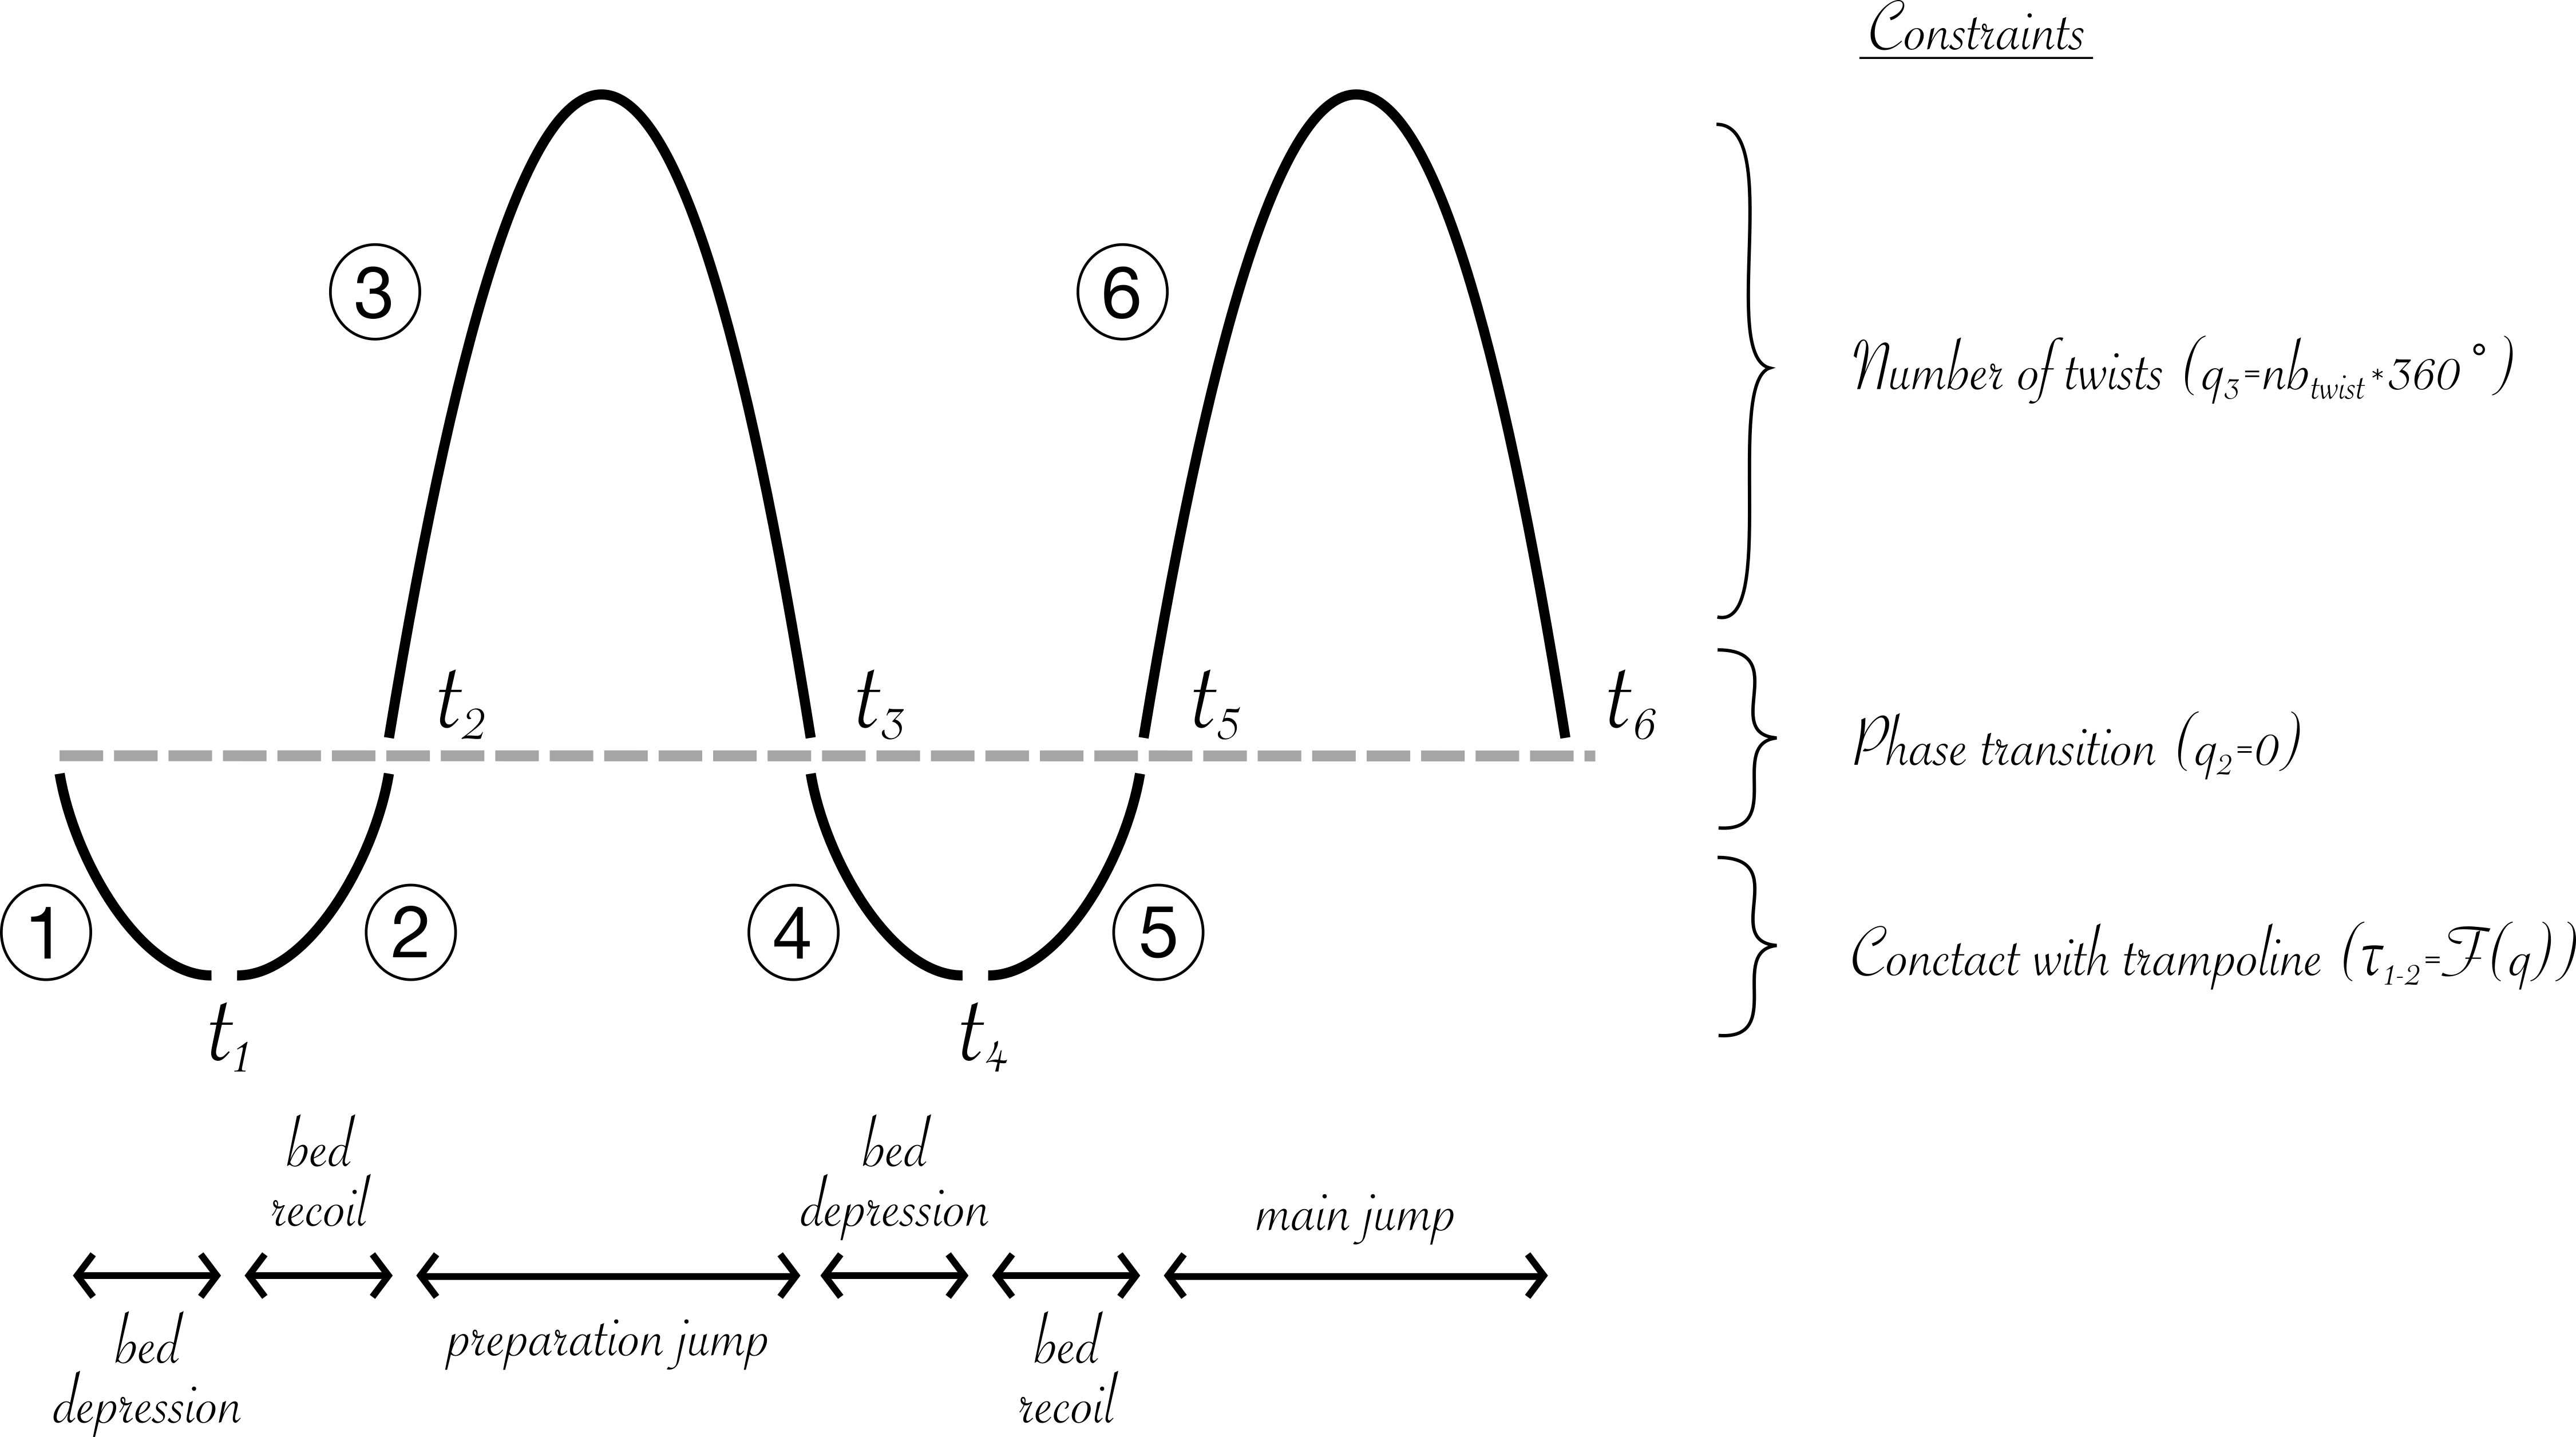
\includegraphics[width=0.5\linewidth]{figures/Model_phases.png}
% \caption{Illustaration of the separation of the OCP in 6 phases.}
% \label{fig:Model_phases}
% \end{figure}


\subsection{Multi-start approach}\label{subsec:2f}
\comEC{départs avant, arrière, avant-arriere, arriere-avant (0, 1, 2, 3, 4, 5 saltos groupé, carpé, tendu) changer la force du modèle}
A multi-start approach was used to explore a wider variety of local optimum \cite{huchez2015local}.
Each OCP (F, B, FB, BF with somersault ranging from 1 to 4) was solved with 50 ??? random initial conditions.
The solution presenting the greatest height for each OCP was saved for later analysis.


\subsection{Biomechanical analysis of the solutions}\label{subsec:2g}
Angular momentum + max CoM height
Deformation history
Faire en sorte que ls force soit appliquée loin du CoM





